% 2009 年广东卷（理科）第 1 题：全集 U 中集合 N、M 的韦恩图，阴影为 N∩M。
% 来源 PDF：.work/ocr-local/sources/2009广东理.pdf
% SHA-256：5256b35235a042e254d36c111af3eda0f5dd8f552664021d0bace5c05582ad04
% 原页：第 1 页（A3 四栏）第 1 栏，印刷页 519。
% 绘制依据：矩形表示 U，左圆 N、右圆 M 相交，交集透镜（N∩M）填灰；
%   原页只在矩形左上角标 U，两圆内分别标 N、M。
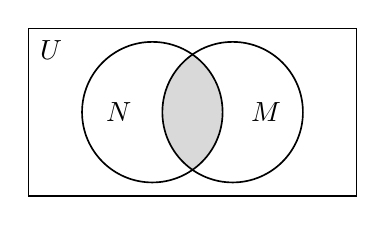
\begin{tikzpicture}[scale=0.85, semithick, every node/.style={inner sep=2pt}]
  \draw (0,0) rectangle (4.9,2.5);
  \node[anchor=north west] at (0.08,2.42) {$U$};
  \begin{scope}
    \clip (1.85,1.25) circle (1.05);
    \fill[gray!30] (3.05,1.25) circle (1.05);
  \end{scope}
  \draw (1.85,1.25) circle (1.05);
  \draw (3.05,1.25) circle (1.05);
  \node at (1.35,1.25) {$N$};
  \node at (3.55,1.25) {$M$};
\end{tikzpicture}
